\begin{abstract}
\textbf{Problem.} Monocular SLAM has no absolute scale of its own. A frozen FM
metric-depth network looks like it could supply one, and is increasingly used as
if it does. We ask the narrow, falsifiable question: \emph{does it actually
transfer metric scale, and if not, what is the smallest fix?}

\textbf{What we found.} On HI-SLAM2 with MapAnything over ten sequences (sixteen
for the gate), it does not, and the reason is structural. The global depth
rescale a metric prior would supply is an exact blind spot of the monocular
factor graph ($3.4\times10^{-13}$ px reprojection change), so no reprojection,
photometric, or prior-consistency residual (and no online estimator) can
observe it. HI-SLAM2 realizes this gauge freedom by median-normalizing the prior
at every keyframe and hard-coding the initial gauge; removing those mechanisms
(a true metric-depth factor, Sec.~\ref{sec:nolocal}) leaves the conclusion unchanged, which is
what makes the diagnosis a property of the monocular graph rather than of one
codebase. No
cheap image signal replaces an anchor: neither cross-view depth consistency nor a
prior-free depth ratio predicts the needed correction, and an online estimator
beats a fixed model on one of three sequences. Two constructive results survive.
A \textbf{trust gate} on the \emph{dispersion} of a short prior-free warm-up ratio
flags when the network's scale is untrustworthy (AUROC 0.97 on sixteen sequences;
the network's own confidence scores 0.44). And a \textbf{trajectory-scale anchor}
recovers scale on all ten validated sequences (mean error 0.024) and thirteen of
sixteen overall, where a depth-mean anchor
fails (mean error 0.306). A trust-gated protocol combining the two cuts mean
trajectory error from 5.9\,m to 0.11\,m on the ten (14.7\,m to 0.33\,m across all
sixteen).

\textbf{What to do.} Treat the metric prior as a sensor to be \emph{audited}, not
trusted: gate its scale on the warm-up dispersion, and if it is trusted, anchor
the gauge to the model. Otherwise spend a sparse, one-shot external metric
measurement (an occasional rangefinder, stereo frame, or fiducial check) to
pin trajectory scale, and use the model for dense structure only. The
identifiability diagnosis and the trajectory anchor generalize across depth
models; the dispersion gate is specific to MapAnything, and GT-free detection of
scale uncertainty remains open.
\end{abstract}

\RALkeywords

\section{Introduction}

Monocular SLAM reconstructs a scene from a single moving camera. Because a
photograph fixes no absolute size, the whole reconstruction is only defined up to
one global factor; we call this the gauge. A reconstruction can be perfectly
self-consistent and still be 3$\times$ too small. Something external must fix the
gauge before the output is metric.

Foundation-model monocular depth networks are an appealing external source. Many
of them, including MapAnything and the metric variants of Depth Anything, predict
depth in metres, and are now dropped into SLAM and Gaussian-splatting pipelines
as if those metres transfer through the pipeline unchanged. This paper asks
whether they do.

\paragraph{Names used throughout.} The frozen depth network is the
\emph{teacher} (MapAnything; DA-V2 Metric-Indoor and DA3METRIC for generality).
The SLAM system it feeds is the \emph{vehicle} (HI-SLAM2). The outside
measurement that pins the global size is the \emph{anchor}; we compare a
\emph{depth-mean} anchor (match the scene's average depth) with a
\emph{trajectory-scale} anchor (match a metric translation to the trajectory).
$r_{init}$ is the median ratio of teacher depth to the system's own depth over a
short prior-free warm-up, and \emph{dispersion} is its spread; AUROC scores the
trust gate (0.5 = chance); ATE is trajectory error in metres after rigid
alignment with scale fixed, so a scale error appears as trajectory error.

\paragraph{Setting and use case.} The camera that runs continuously is monocular,
but in many robotics deployments a metric measurement is available
\emph{occasionally}: a downward rangefinder or imaging sonar~\cite{yang2022sonar},
a stereo or RGB-D frame that is briefly mounted or momentarily
reliable~\cite{murartal2017}, a fiducial at a docking station~\cite{olson2011},
or GNSS in good sky~\cite{wu2017vins}. Fusing episodic measurements of this kind
is the classical intermittent-observation setting~\cite{sinopoli2004}. We take
that literally: the protocol below spends roughly twenty sparse keyframe pairs
\emph{once} at startup to fix the gauge, then tracks with the monocular camera and
the frozen FM prior for dense geometry. This is not continuous multi-sensor
fusion; it is a bounded, one-shot metric check placed exactly where monocular
SLAM is structurally blind.

\paragraph{What we did, and the short answer.} We study one concrete SLAM system
(HI-SLAM2) and one frozen depth model (MapAnything) over ten sequences (sixteen for the gate), then
repeat the key test with two more depth models (DA-V2 Metric-Indoor, DA3METRIC)
to see what generalizes; KITTI is a documented out-of-domain control, reported as
a limit of the SLAM system rather than a result about depth models. The metric
scale does not transfer, and the reason is not that one system is buggy: it is an
\emph{identifiability} problem. The SLAM system realizes the monocular gauge
freedom by normalizing the prior at every keyframe and fixing the initial gauge
to a constant, so the model's metres are discarded before they can matter; we
show the same holds after those mechanisms are removed (Sec.~\ref{sec:nolocal}). You must supply
one external metric number. Once you do, the pipeline is metric to the accuracy
of that number. The practical version is a trust gate plus a trajectory-scale
anchor.

\paragraph{What we found (in order of the paper).} (i) The system discards the
prior's scale by construction: swapping depth networks changes nothing (0.316
vs.\ 0.339), because a hard-coded gauge constant dominates. (ii) Anchoring the
gauge to the model recovers scale in-domain to the model's own bias (0.907
vs.\ 0.903) but transfers the wrong scale out of distribution (EuRoC 0.13--0.21).
(iii) No free signal replaces the anchor, and an online estimator beats a fixed
model on 1 of 3 sequences. (iv) The \emph{spread} of the warm-up ratio is a usable
trust gate \emph{for MapAnything} (AUROC 0.97 over sixteen sequences; the model's
own confidence scores 0.44). (v) The right anchor is trajectory scale, not depth mean: the latter fails
(0.70/0.86/0.86 on three EuRoC sequences), the former recovers all ten (mean
error 0.024) and thirteen of sixteen, failing only on difficult low-parallax
sequences. (vi) A deliberate 25\% local FM-depth step is absorbed by both the
stock and the metric-factor vehicle: there is no live local lever. (vii) Gate + anchor cut mean trajectory error
5.9\,m $\to$ 0.11\,m; the diagnosis and anchor hold across three models, the
specific gate does not.

\paragraph{Contributions.} (1)~A measured identifiability result: the global
metric-scale direction is an exact null direction of the monocular factor graph,
so no reprojection, photometric, or prior-consistency residual (nor any online
estimator) can recover it without an absolute metric measurement
(Sec.~\ref{sec:gauge}; confirmed after removing the vehicle's keyframe normalization, Sec.~\ref{sec:nolocal}).
(2)~A universal fallback: a trajectory-scale anchor that recovers scale on
thirteen of sixteen sequences, where a depth-mean anchor fails (Sec.~\ref{sec:anchor}).
(3)~A demonstrator and a fence: model-internal confidence is consistently useless
for scale trust (AUROC 0.44; a constant 1.0 for DA3METRIC), while the dispersion
of the initial ratio is a viable gate \emph{for MapAnything} (AUROC 0.97);
GT-free scale-uncertainty detection remains open and model-dependent
(Secs.~\ref{sec:gate}--\ref{sec:model}).

\section{Related Work}

We position this as a \emph{measured identifiability result and a protocol}, not
a new SLAM back-end.

\noindent\textbf{Positioning.} The FM-prior SLAM line
(HI-SLAM2~\cite{hislam2}, CF2-SLAM~\cite{cf2slam}, PRISM-SLAM~\cite{prismslam},
Scalix~\cite{scalix}, VGGT-SLAM 2.0~\cite{vggtslam2}) reaches metric monocular
output by \emph{adopting} the teacher's scale, either directly or through a
calibrated, probabilistic factor, and works when the teacher is in-domain. None
of these can detect when adoption fails: PRISM's ray-distance factor makes the
metric scale Fisher-identifiable but assumes the prior carries the right metres;
Scalix treats a \emph{learned} per-frame scale uncertainty as an independent
measurement; CF2-SLAM calibrates coverage, not the scale value. Our audit
supplies the missing failure statement (which direction is unobservable,
measured), our \textbf{trust gate} supplies the missing failure detector (before
deployment, from a prior-free reference), and our \textbf{anchor} supplies the
missing fallback (pin trajectory scale when the gate rejects). The consistency
accounting we propose is the missing evidence for the part of the error that
\emph{is} observable.

\begin{itemize}
\item \textbf{Scale-aware and metric SLAM.} Several concurrent systems add scale
  handling or calibration to SLAM and SLAM+GS pipelines (e.g.\
  Scalix~\cite{scalix}; the FM-based line: HI-SLAM2~\cite{hislam2},
  CF2-SLAM~\cite{cf2slam}, PRISM-SLAM~\cite{prismslam}, VGGT-SLAM
  2.0~\cite{vggtslam2}). We do not claim those mechanisms.
\item \textbf{FM depth priors.} We study metric-depth models as
  geometry/Gaussian priors; MapAnything~\cite{mapanything} is our frozen teacher,
  with DA-V2 Metric~\cite{depthanythingv2} and DA3METRIC~\cite{da3} for
  generality. Other prior sources include feed-forward geometry
  models~\cite{vggt,vggtslam} and deep monocular odometry with a learned
  uncertainty~\cite{d3vo}; our audit applies to any of them.
\item \textbf{Observability.} The similarity gauge and monocular scale
  unobservability are classical. We give the concrete consequence for FM depth
  priors and a numeric certificate, plus its low-parallax face. The
  visual-inertial line~\cite{merrill,hailu,hdvio2} estimates learned-depth scale in
  \emph{initialization} because the IMU makes scale observable, the external
  observable pure monocular SLAM lacks, and exactly what our anchor must supply.
\end{itemize}

We do not claim to introduce metric SLAM, learned covariance~\cite{macvo}, or
scale-aware factor graphs, nor online-learned model parameters for
odometry~\cite{okawara}; this is not a bug report about HI-SLAM2: its
normalization lines instantiate a gauge freedom that any anchor-free monocular
pipeline has, as confirmed after they are removed (Sec.~\ref{sec:nolocal}).

\section{How the System Handles Depth, and Why Scale is a Blind Spot}

\subsection{The setup}

HI-SLAM2 is monocular factor-graph SLAM with a dense depth prior fed to a
depth-only bundle adjustment at a weight of $0.01$. The depth prior comes from a frozen map of
depth images (one per frame) produced by the teacher, in the system's working
resolution.

\subsection{The gauge argument, and a numeric check}
\label{sec:gauge}

We state the fact we rely on once, as a proposition with a one-paragraph proof,
because the corollary (not the proposition) is what the paper uses. The
similarity gauge is classical; nothing below is claimed as new mathematics.

\medskip
\noindent\textbf{Proposition 1 (gauge null direction).} \emph{Take a pixel with
depth $z_i$, intrinsics $K$, and relative pose $(R,t)$. The reprojection residual
of its backprojected point is invariant to the joint rescaling
$(t,z)\to\lambda(t,z)$ for every $\lambda>0$.}

\smallskip
\noindent\emph{Proof sketch.} Backproject $X_i = z_i K^{-1}[u_i,1]$ and project
forward as $X_j = R X_i + t$. Under the joint rescale, $X_j \to \lambda X_j$, and
projection divides out that common scale, so the image point $u_j$ does not move,
while the depth it implies grows by $\lambda$. Only the ratio $t/z$ enters
the residual. Depth-only rescaling ($z$ alone, $t$ fixed) is not a symmetry,
because it changes that ratio. \hfill$\square$

\smallskip
\noindent\textbf{Corollary 1.} \emph{Any estimator state whose update direction is
the joint rescale (a global depth-scale ``bias'' state) lies in the exact
null space of the residual and is structurally unobservable. In pure monocular
SLAM such a state carries no information and should not be estimated; the global
metric scale can be set only by an external metric reference.} This corollary is
the paper's diagnosis: it is \emph{why} the trust gate needs a prior-free
reference and \emph{why} an anchor is mandatory, and it bounds what any online
estimator can certify. Corollary~1 is a statement about the \emph{monocular factor
graph}, not about a particular implementation: reprojection, photometric, and
prior-consistency residuals are all invariant to the joint $(t,z)$ rescale, so no
arrangement of them, including a metric-depth factor at full weight, observes
the scale direction. A graph with no absolute metric measurement retains this
gauge freedom, and an estimate initialized in that gauge stays there.

We checked the proposition numerically. A joint $(t,z)$ rescale changes the
reprojected point by $3.4\times10^{-13}$ px (numerical zero). A depth-only rescale
($z$ alone, $t$ fixed) changes it by 215.6 px, and a small rotation perturbation
by 6.8 px, so the test is sensitive. The three numbers together are the
certificate: the joint direction is null, the depth-only direction is not, and
the measurement could have seen a difference if there were one.

\subsection{How the shipped vehicle realizes the gauge freedom}

Two mechanisms are load-bearing. First, at every keyframe the prior is
median-normalized to the system's own disparity (the ratio of the two medians).
Second, at warm-up the mean depth is pinned once to a constant (a scale
multiplier of 2.0). Together these mean the teacher's absolute scale never reaches the estimate, and
the global gauge is set once and frozen. These lines are \emph{how this vehicle
realizes} the gauge freedom, not the result: Sec.~\ref{sec:nolocal} removes them by wiring the
prior as a true metric-depth factor, and the global conclusion is unchanged,
exactly as the structural argument predicts.

\section{Method}

\begin{enumerate}
\item \textbf{Audit.} Serve a frozen teacher and confirm the realized scale does
  not depend on which teacher it is (we swap Omnidata for MapAnything and get the
  same result).
\item \textbf{Gauge anchor.} Replace the hard-coded gauge constant with the
  teacher's mean metric depth. The measured relation is
  $\mathrm{scale}(a)=\mathrm{scale}(1)/a$, so the oracle anchor is
  $a=\mathrm{scale}(1)$. In-domain this makes the reconstruction metric to the
  teacher's own accuracy.
\item \textbf{Trust gate.} From a short \emph{prior-free} warm-up, compute
  $r_{init}=\mathrm{median}(D_{teacher}/D_{backend})$ and its dispersion over the
  window. Trust the teacher's scale when the dispersion is low.
\item \textbf{Sparse anchor protocol (opportunistic sensor fusion).} When the
  gate rejects a sequence (or it is known to be out of distribution), pin metric
  \textbf{trajectory scale} from one short external metric translation (RGB-D or
  stereo PnP, matched to the backend trajectory) and use the teacher for dense
  structure only. A depth-mean anchor is not sufficient.
\end{enumerate}

\section{Experiments}

\paragraph{Setup.} HI-SLAM2 (torch 2.1.2) plus frozen MapAnything depth maps over
ten sequences: five from the TUM RGB-D benchmark~\cite{tumrgbd} (f1\_xyz,
f1\_desk, fr2\_xyz, fr2\_desk, fr3\_long\_office\_household) and five from
EuRoC~\cite{euroc} (MH\_01, MH\_02, V1\_01, V1\_02, V2\_01). All
injection is external (no edits to the SLAM code); ground truth is TUM registered
depth and TUM/EuRoC trajectories.

\paragraph{Vehicle-domain control.} KITTI-800~\cite{kitti} (odometry 00, first 800 frames,
outdoor driving) is a documented limit of the \emph{SLAM system}, not a result
about depth models: stock HI-SLAM2 gives umeyama scale 4.74 (ATE 10.3\,m) and the
FM-wired run 3.86 (ATE 13.9\,m). Both are wrong by roughly 4$\times$ regardless
of the prior, so we exclude KITTI from the prior claims.

\subsection{The gauge dominates; anchoring recovers scale in-domain}

\begin{table}[t]
\centering
\caption{Umeyama scale (est$\to$GT) before and after anchoring the gauge to the
teacher, and the teacher's own average bias; ``fixed gauge'' pins mean depth to
2.0\,m.}
\label{tab:indomain}
\small
\begin{tabular}{@{}lccc@{}}
\toprule
sequence & fixed gauge & anchored & teacher bias \\
\midrule
f1\_xyz & 0.442 & \textbf{0.907} & 0.903 \\
f1\_desk & 0.505 & \textbf{1.063} & 0.907 \\
MH\_01 & 0.316 & \textbf{0.132} & out of distribution \\
V1\_02 & 0.192 & \textbf{0.210} & out of distribution \\
\bottomrule
\end{tabular}
\end{table}

Table~\ref{tab:indomain} shows the effect. On TUM, anchoring recovers the teacher's own accuracy (0.907 vs.\ 0.903): the
dominant error was the hard-coded gauge, not the network. On EuRoC the teacher's
scale is itself wrong, so the same anchor transfers the wrong metres. The gauge
law is linear to measurement precision: anchoring f1\_xyz at 1.1 gives
$0.907/1.1=0.825$ (measured 0.825) and f1\_desk at 0.8 gives $1.063/0.8=1.327$
(measured 1.327). Read the adopted scale against the teacher-bias column, not
against 1.0: the residual is the teacher's bias faithfully inherited.

\subsection{No free signal replaces the anchor}

We looked for a signal already in the data that would predict the correction, so
an anchor would not be needed. The candidate was the warm-up ratio
$r_{init}=\mathrm{median}(D_{teacher}/D_{backend})$, computed from a prior-free
run at the fixed gauge. Its \emph{average} versus the oracle anchor is in
Table~\ref{tab:ratio}.

\begin{table}[t]
\centering
\caption{The average warm-up ratio does not predict the needed anchor: the
pairwise sign agrees three times and disagrees three times.}
\label{tab:ratio}
\small
\begin{tabular}{@{}lccc@{}}
\toprule
sequence & $r_{init}$ & oracle anchor & domain \\
\midrule
f1\_xyz & 0.478 & 0.907 & TUM \\
f1\_desk & 0.512 & 1.063 & TUM \\
MH\_01 & 0.734 & 0.132 & EuRoC \\
V1\_02 & 0.189 & 0.210 & EuRoC \\
\bottomrule
\end{tabular}
\end{table}

The simple physical model ($r=\beta/\gamma$, anchor${}=1/\beta$) predicts the
anchor should fall as $r$ rises, but only if the reference gauge is the same in
every domain. It is not: the pairwise signs agree three times and disagree three
times, so there is no usable monotone relation, and a fit calibrated on one
domain extrapolates $18\times$ wrong on MH\_01. A five-arm ladder (fixed gauge,
in-domain, frozen calibration, online adaptation, oracle) tells the same story in
scale error (Table~\ref{tab:ladder}): the online arm beats the frozen arm on only
one of three informative sequences. \textbf{We rejected the online-transfer
route.}

\begin{table}[t]
\centering
\caption{Scale error of the five-arm ladder. Online adaptation beats frozen
calibration on only one of three informative sequences.}
\label{tab:ladder}
\small
\begin{tabular}{@{}lccccc@{}}
\toprule
sequence & fixed gauge & in-domain & frozen & online & oracle \\
\midrule
f1\_xyz & 0.496 & 0.093 & 0.107 & 0.177 & 0.000 \\
f1\_desk & 0.403 & 0.063 & 0.047 & 0.130 & 0.000 \\
MH\_01 & 0.661 & 0.868 & 0.870 & 0.682 & 0.000 \\
V1\_02 & 0.808 & 0.790 & 0.794 & 0.977 & 0.000 \\
\bottomrule
\end{tabular}
\end{table}

\subsection{Dispersion is a usable trust gate (for MapAnything)}
\label{sec:gate}

The average of $r_{init}$ does not help, but its spread does. On ten sequences,
with an out-of-distribution label defined purely from metric truth
($|\mathrm{scale}-1|>0.30$), the split is in Table~\ref{tab:label}.

\begin{table}[t]
\centering
\caption{Trust label is defined from metric truth, not from the domain.}
\label{tab:label}
\small
\setlength{\tabcolsep}{4pt}
\begin{tabular}{@{}lp{0.64\linewidth}@{}}
\toprule
label & sequences \\
\midrule
trust (6) & f1\_xyz, f1\_desk, fr2\_desk, fr3\_long\_office, V1\_01, V2\_01 \\
out of dist.\ (4) & fr2\_xyz, MH\_01, MH\_02, V1\_02 \\
\bottomrule
\end{tabular}
\end{table}

Notice the label is not the domain: V1\_01 and V2\_01 are EuRoC yet
trustworthy, and fr2\_xyz is TUM yet out of distribution. The gate, for which low
dispersion means ``trust'', scores \textbf{AUROC 0.917} (threshold 0.0625,
accuracy 0.90), with one conservative false rejection (V2\_01). The network's own
confidence is useless for this: AUROC 0.44. It is confidently wrong.

The gate is not an artifact of small samples or of the warm-up window. A
sequence-level bootstrap gives a mean of 0.918 with 95\% CI [0.667, 1.000], and
leave-one-out never drops below 0.889. Recomputing every sequence's dispersion
from a \emph{fixed} frame budget (the minimum 11 frames, versus the actual
11--106) leaves the AUROC at 0.917, and the correlation between dispersion and
frame count is only $-0.26$. The AUC is flat across windows from 10 to 100 frames
(0.833 at 5). \textbf{The gate reads the domain shift, not the sample size.}

Adding the six remaining EuRoC sequences (\textbf{16 total, 7 gate-positive})
raises the AUROC to \textbf{0.968} (bootstrap 95\% CI [0.859, 1.000];
leave-one-out $\ge0.963$; fixed frame budget 0.968, so this is the same
statistic, not a length effect). The added sequences are informative, not filler:
MH\_03/04/05 are correctly flagged out of distribution (dispersion 0.51/0.64/0.80)
and V1\_03/V2\_02/V2\_03 trusted (0.09/0.06/0.02). Caveat: the added reference
runs use a GS-free, 300-frame vehicle configuration, so this compares the
\emph{init-window statistic} across a slightly different backend setup.

\subsection{Generalizes across models, but the gate is model-specific}
\label{sec:model}

We repeated the test with two more metric depth models.
\textbf{DA-V2 Metric-Indoor-Large}~\cite{depthanythingv2} is less metric in many
more sequences (gauge scale 0.557/0.738 on f1\_xyz/f1\_desk; 6 of 10 out of
distribution, including two TUM sequences). \textbf{DA3METRIC-LARGE}~\cite{da3}
is near-metric in-domain but systematically over-estimates by 15--43\% (5 of 10
out of distribution), and is badly off on EuRoC (0.23--0.26). Every model
confirms the identifiability diagnosis, and every model fails differently:
DA3METRIC even emits a constant confidence of 1.0, so confidence is never a
scale-trust signal. The \emph{gate}, however, does not transfer
(Table~\ref{tab:models}).

\begin{table}[t]
\centering
\caption{Gate AUROC per depth model (ten sequences). Bootstrap CIs overlap
because there are only 4--6 OOD cases; leave-one-out separates them.}
\label{tab:models}
\footnotesize
\setlength{\tabcolsep}{4pt}
\begin{tabular}{@{}lccc@{}}
\toprule
depth model & AUROC & 95\% CI & LOO \\
\midrule
MapAnything & \textbf{0.917} & [0.667, 1.000] & 0.889--1.000 \\
DA-V2 Metric-Indoor & 0.625 & [0.167, 1.000] & 0.500--0.778 \\
DA3METRIC-LARGE & 0.600 & [0.160, 1.000] & 0.500--0.700 \\
\bottomrule
\end{tabular}
\end{table}

\noindent The point estimates separate (0.92 versus about 0.6), and the
fixed-budget check gives the same number in each case, so this is not a length
artifact. The bootstrap intervals overlap because there are only 4--6
out-of-distribution cases per model; the sharper statistic is leave-one-out,
where both alternative models fall to 0.50 (chance) while MapAnything never drops
below 0.889.

Allowing each model its own decision rule does not close the gap. Sweeping the
positive-class threshold $\tau$ (defining ``scale wrong'' as $|$scale$-1|>\tau$)
and calibrating $\tau$ per model, MapAnything reaches AUROC \textbf{1.00} at a
stable $\tau^\ast=0.20$ (leave-one-sequence-out $\tau^\ast=0.215\pm0.045$), while
DA-V2 and DA3METRIC reach only 0.875 ($\tau^\ast=0.475$) and 0.810
($\tau^\ast=0.700$) at \emph{unstable} $\tau^\ast$ (LOSO std 0.144 and 0.135,
bootstrap CIs including 0.5). A per-model constant cannot rescue a weak ranking;
the dispersion construct itself is MapAnything-specific here.

The split to carry away: \textbf{the identifiability diagnosis and the trajectory
anchor are universal; the dispersion gate is a MapAnything-specific demonstration
that the construct can work, not a universal detector.} Model-internal confidence
is consistently uninformative (MapAnything 0.44; DA3METRIC emits a constant 1.0),
and GT-free detection of scale uncertainty remains an open, model-dependent
problem.

\subsection{The right anchor is trajectory scale, not depth mean}
\label{sec:anchor}

With the gauge law, an \emph{oracle} anchor $a=a_{gt}(1+\epsilon)$ gives scale
error $\epsilon/(1+\epsilon)$ on every sequence (e.g.\ 0.000/0.091/0.167/0.231
for $\epsilon={}$0.0/0.1/0.2/0.3), independent of the scene. The question is
whether a \emph{realistic} anchor realizes it. A depth-mean anchor (match the
scene's average depth) does not. Measured with real backend runs on all ten
sequences, using the dataset's own sensor (TUM RGB-D or EuRoC stereo), the
comparison is in Table~\ref{tab:anchor}.

\begin{table}[t]
\centering
\caption{Anchor error per sequence for a depth-mean versus a trajectory-scale
anchor, with the teacher's own error.}
\label{tab:anchor}
\footnotesize
\setlength{\tabcolsep}{4pt}
\begin{tabular}{@{}lcccc@{}}
\toprule
sequence & sensor (m) & teacher & depth-mean & traj. \\
\midrule
f1\_xyz & 1.128 & 0.093 & 0.113 & \textbf{0.009} \\
f1\_desk & 1.163 & 0.063 & 0.020 & \textbf{0.069} \\
fr2\_xyz & 1.330 & 0.359 & 0.029 & \textbf{0.044} \\
fr2\_desk & 1.699 & 0.192 & 0.178 & \textbf{0.005} \\
fr3\_long & 2.532 & 0.005 & 0.106 & \textbf{0.010} \\
MH\_01 & 2.275 & 0.868 & 0.704 & \textbf{0.004} \\
MH\_02 & 3.248 & 0.903 & 0.856 & \textbf{0.047} \\
V1\_01 & 2.216 & 0.107 & 0.039 & \textbf{0.011} \\
V1\_02 & 2.696 & 0.790 & 0.857 & \textbf{0.013} \\
V2\_01 & 3.414 & 0.203 & 0.156 & \textbf{0.031} \\
\midrule
\textbf{mean (10)} & & 0.358 & 0.306 & \textbf{0.024} \\
\bottomrule
\end{tabular}
\end{table}

\noindent The depth-mean anchor is no better than the teacher overall (0.306 vs.\
0.358), inconsistent in-domain (0.020--0.178), and catastrophic on three EuRoC
sequences (0.70/0.86/0.86). The reason is the one we found earlier: the average
depth that makes the \emph{sensor} metric and the average depth that makes the
\emph{trajectory} metric are different, badly so out of distribution. A
trajectory-scale anchor, a metric translation matched to the backend trajectory,
recovers all ten sequences (mean \textbf{0.024}), using 11--27 matched pairs each
with a bootstrap interval. Dense short-baseline pairs across the trajectory also
remove our earlier failure cases (f1\_desk is now 0.069, not degenerate; V1\_02
rests on 12 pairs, not 1).

Extending the anchor to the six remaining EuRoC sequences tests where it stops
working. It accepts \textbf{13 of the 16} sequences (mean error \textbf{0.021},
worst 0.069); the three it rejects are MH\_04, MH\_05 and V2\_03, the hardest
sequences, where matched stereo pairs are poorest and the pair-ratio interval
widest (V2\_03 fails on a CI half-width above 0.25, the other two on scale). The
three new sequences it does recover have teacher errors of 0.93/0.03/0.11 and
anchor errors of 0.003/0.010/0.010. This is the anchor's practical low-parallax
limit (Sec.~\ref{sec:lowpar}): it is exact where matched translation exists and
refuses where it does not.

\subsection{The low-parallax limit, stated exactly}
\label{sec:lowpar}

The trajectory anchor needs translation, and the underlying limit is exact.
Holding the pose fixed, a 10\% depth-scale error changes the reprojection by
$2.3\times10^{-13}$ px at zero translation (depth is a pure gauge there), and the
change grows monotonically with baseline: 0.007 px at $|t|=10^{-4}$, 0.74 at
0.01, 7.0 at 0.1, 42 at 1.0. Real keyframe baselines are far from this limit: the
anchor's scale stays within a few percent across baseline terciles, with mean
interval half-width 0.147 (low) versus 0.133 (high). \textbf{So the
teacher-only failure is a fact about identifiability, not a side effect of low
parallax.}

\subsection{The sparse-anchor protocol, measured in metres}
\label{sec:protocol}

Composing the gate (threshold 0.0625) with the trajectory anchor gives the
paper's practical result, measured as rigid-aligned trajectory error so that a
scale error shows up as metric error:

\begin{itemize}
\item \textbf{Teacher scale only (the naive default):} mean scale error 0.358,
  mean ATE \textbf{5.94\,m}.
\item \textbf{Gate + trajectory anchor:} mean scale error 0.060, mean ATE
  \textbf{0.11\,m}.
\end{itemize}

\noindent The right way to read this is \textbf{catastrophe prevention, not a
marginal ATE improvement}. ``Teacher scale only'' is not a weak baseline: it is
the default of deploying an FM metric-depth prior and trusting its metres
everywhere. On the four out-of-distribution sequences it produces trajectory
errors of tens of metres. The protocol does not make an already-good system
slightly better; it turns a silent, unbounded failure into a bounded one.

\noindent Five sequences are trusted and use the teacher's scale directly (mean
error 0.092). The other five are rejected and use the trajectory anchor;
teacher-only would have erred 0.625 on them (0.730 on the four truly
out-of-distribution cases). The four worst cases are all recovered: MH\_01
$30.0\to0.05$\,m, MH\_02 $21.4\to0.11$\,m, V1\_02 $6.7\to0.07$\,m, fr2\_xyz
$0.14\to0.01$\,m. The gate is conservative but safe, and the anchor makes a false
rejection cost nothing.

\noindent Applied across all sixteen sequences, including the three where the
anchor cannot be validated, the gate+anchor protocol still cuts mean rigid ATE
from \textbf{14.7\,m to 0.33\,m} (scale error 0.417$\to$0.083; the
sixteen-sequence gate uses its own threshold 0.0979, the ten uses 0.0625). The
residual is concentrated entirely in the difficult cases: MH\_04 $66.7\to2.0$\,m
and MH\_05 $59.5\to1.5$\,m, where the anchor itself fails, while the third anchor
failure, V2\_03, is trusted by the gate and stays at its teacher error
(0.36\,m). The ten-sequence result is the clean statement; the sixteen-sequence
run shows the protocol degrades boundedly rather than silently.
Figs.~\ref{fig:summary} and \ref{fig:tier12} summarize the gate and protocol.
Table~\ref{tab:protocol} lists the per-sequence outcome; the protocol spends 264
sparse pairs in total (11--27 per sequence).

\begin{table*}[t]
\centering
\caption{Per-sequence outcome of the gate$+$anchor protocol over all sixteen
sequences. ``disp.'' is the warm-up dispersion $\sigma_{\log}$ (threshold
0.0979), ``src'' the scale source finally used, and ATE is rigid-aligned
trajectory error in metres. The eight trusted sequences keep the teacher's
scale; the eight rejected ones take the trajectory anchor. The two worst
rejections (MH\_04, MH\_05) are the anchor's own failures.}
\label{tab:protocol}
\footnotesize
\setlength{\tabcolsep}{6pt}
\begin{tabular}{@{}lcccccc@{}}
\toprule
sequence & disp. & gate & src & pairs & ATE teacher (m) & ATE protocol (m) \\
\midrule
f1\_xyz & 0.012 & trust & FM & 23 & 0.020 & \textbf{0.020} \\
f1\_desk & 0.022 & trust & FM & 13 & 0.055 & \textbf{0.055} \\
fr2\_xyz & 0.474 & reject & anchor & 18 & 0.138 & \textbf{0.012} \\
fr2\_desk & 0.061 & trust & FM & 11 & 0.464 & \textbf{0.464} \\
fr3\_long & 0.010 & trust & FM & 13 & 0.016 & \textbf{0.016} \\
MH\_01 & 0.240 & reject & anchor & 27 & 30.029 & \textbf{0.050} \\
MH\_02 & 0.288 & reject & anchor & 17 & 21.429 & \textbf{0.109} \\
MH\_03 & 0.510 & reject & anchor & 19 & 49.454 & \textbf{0.046} \\
MH\_04 & 0.642 & reject & anchor & 25 & 66.731 & \textbf{1.994} \\
MH\_05 & 0.802 & reject & anchor & 17 & 59.457 & \textbf{1.511} \\
V1\_01 & 0.020 & trust & FM & 11 & 0.173 & \textbf{0.173} \\
V1\_02 & 0.621 & reject & anchor & 12 & 6.664 & \textbf{0.073} \\
V1\_03 & 0.094 & trust & FM & 15 & 0.084 & \textbf{0.084} \\
V2\_01 & 0.382 & reject & anchor & 13 & 0.369 & \textbf{0.090} \\
V2\_02 & 0.059 & trust & FM & 15 & 0.265 & \textbf{0.265} \\
V2\_03 & 0.022 & trust & FM & 15 & 0.361 & \textbf{0.361} \\
\midrule
\textbf{mean} & & & & 16.5 & 14.732 & \textbf{0.333} \\
\bottomrule
\end{tabular}
\end{table*}

\noindent\textbf{What the protocol costs.} The anchor needs only 11--27 sparse
keyframe pairs, applied \emph{once} at startup, and the gate needs only a short
prior-free warm-up: roughly twenty measurements to bound the monocular failure,
after which tracking is pure monocular with the FM prior supplying dense
geometry. The metric source can be opportunistic (a rangefinder or sonar, a
brief stereo or RGB-D frame, a docking fiducial, GNSS) and is not committed to
the front end~\cite{sinopoli2004,yang2022sonar,murartal2017,olson2011,wu2017vins}.
The one case this does not help is a platform whose \emph{only} sensor is RGB-D;
then monocular SLAM has no advantage and the protocol is moot.

\subsection{The global gauge has no local lever}
\label{sec:nolocal}

If the global gauge is a blind spot, perhaps local model scale is trackable. It
is not, in either vehicle. In the shipped system a deliberate 25\% step in the
model's depth from frame 400 leaves the global scale unmoved (0.8246 vs.\ 0.8252)
and the per-keyframe depth pass-through at the noise floor ($\sim$0.0016),
because of the per-keyframe renormalization. Wired as a true \textbf{metric-depth
factor} (scale grid removed, prior entering at its own metres), the global result
is unchanged: the scalar and confidence-weighted arms sit at or slightly worse
than stock (mean $|$scale$-1|=0.523$ vs.\ 0.409) and never approach the anchored
result; raising the prior weight $\alpha$ from 0.01 to 10 reproduces the
$0.44\to0.50$ shift but never reaches the teacher's 0.90 (Table~\ref{tab:arms}).
\textbf{The failure
survives removing the per-keyframe normalization entirely, so it is the gauge
null of the monocular graph, not HI-SLAM2's implementation.} A deliberate local
step is likewise absorbed by both vehicles, and per-pixel confidence weighting
changes shape, not scale.

\begin{table}[t]
\centering
\caption{Umeyama scale (est$\to$GT) per metric-factor arm. The metric residual
does not make the global gauge observable: the scalar and confidence-weighted
arms never approach the anchored result.}
\label{tab:arms}
\scriptsize
\setlength{\tabcolsep}{4pt}
\begin{tabular}{@{}lccccc@{}}
\toprule
sequence & stock & scalar & conf. & metric$+$anch. & anchor only \\
\midrule
f1\_xyz & 0.505 & 0.505 & 0.499 & 0.896 & 0.907 \\
f1\_desk & 0.597 & 0.577 & 0.538 & 0.964 & 1.063 \\
fr2\_xyz & 0.680 & 0.748 & 0.750 & 0.708 & 0.641 \\
fr2\_desk & 1.000 & 1.088 & 1.090 & 0.823 & 0.808 \\
fr3\_long & 1.132 & 1.450 & 1.432 & 1.288 & 1.005 \\
MH\_01 & 0.339 & 0.270 & 0.353 & 0.133 & 0.132 \\
MH\_02 & 0.231 & 0.271 & 0.265 & 0.125 & 0.097 \\
V1\_01 & 1.065 & 1.333 & 1.351 & 1.403 & 1.107 \\
V1\_02 & 0.192 & 0.212 & 0.242 & 0.036 & 0.210 \\
V2\_01 & 1.439 & 1.881 & 2.008 & 1.607 & 1.203 \\
\midrule
mean & 0.409 & 0.517 & 0.523 & 0.462 & 0.358 \\
\bottomrule
\end{tabular}
\end{table}

\subsection{The observable half: a scalar calibrates; a per-regime extension is fragile}
\label{sec:observable}

A scalar variance scale on the observable half can be calibrated online. We
weight the metric-factor residual by the teacher's confidence and adapt a
variance scale online by covariance matching~\cite{mehra}, reporting the depth-channel NIS
(target 1; we use the median over solves because rare diverging solves dominate
the mean, on MH\_01 a few solves reach NIS $>10^5$). Frozen confidence weighting
is miscalibrated by a sequence-dependent factor: median NIS 0.477 (f1\_xyz),
0.074 (f1\_desk), 0.021 (MH\_01), 0.082 (V1\_02), so no single temperature
covers all. A scalar adaptation brings every sequence closer to 1
(1.380/0.469/0.033/0.025), closer than frozen on all four, but on the
extreme-OOD MH\_01 it pins its floor ($c=c_{\min}=0.2$) at NIS 0.033, because
the miscalibration is not a global temperature.

Replacing the scalar with $K{=}3$ confidence-quantile regimes (edges calibrated
from the first 60 solves, then edges and $c_k$ frozen at 300 solves, held-out on
later tracking solves) passes the pre-registered test in this one configuration
(Table~\ref{tab:sigma}): per-regime $\sigma$ is closer to 1 than the scalar on
all three shifted sequences and reduces the mean per-regime deviation
$|\mathrm{NIS}_k-1|$ on all four. \textbf{It is not robust.} The pre-registered
$K$-sensitivity ($K\in\{2,4\}$) fails: unguarded, K2/K4 hung in the backend on
both shifted sequences, and the surviving K3 pins the guard floor ($c_k=0.05$)
and diverges on 11\% of held-out MH\_01 solves. Re-running K2/K3/K4 under a
stability guard ($c_{lo}=0.2$, time-capped) makes every arm converge but
\emph{erases the calibration gain} (MH\_01 K3 median 0.032 and V1\_02 K3 median
0.019, versus 0.504/0.615 unguarded). So per-regime $\sigma$ is a single fragile
configuration, not a mechanism; only the scalar adaptation is robust. The
calibration is also \textbf{domain-specific}: freezing the TUM-fitted scalar and
applying it to EuRoC leaves held-out NIS at 0.03--0.09, far from 1, so the
observable half must be re-calibrated per domain. Depth-channel NIS is circular
for absolute scale by construction.

\begin{table}[t]
\centering
\caption{Scalar versus $K{=}3$ per-regime adaptation: depth-channel median NIS
(target 1) and per-regime NIS. Per-regime is closer to 1 but not robust to $K$.}
\label{tab:sigma}
\footnotesize
\setlength{\tabcolsep}{3pt}
\begin{tabular}{@{}lccccc@{}}
\toprule
sequence & scalar med. & regime med. & scalar NIS$_k$ & regime NIS$_k$ \\
\midrule
f1\_xyz & 1.380 & 1.315 & [0.60,2.00,2.78] & [1.33,1.34,1.24] \\
f1\_desk & 0.469 & 0.707 & [0.12,0.37,1.05] & [0.50,0.36,0.67] \\
MH\_01 & 0.033 & 0.504 & [0.01,0.01,0.04] & [0.04,0.07,0.67] \\
V1\_02 & 0.025 & 0.615 & [0.01,0.01,0.03] & [0.16,0.17,0.64] \\
\bottomrule
\end{tabular}
\end{table}

Finally, the gate is \textbf{blind to a constant teacher bias}. Rebuilding the
teacher with perturbed intrinsics ($fx, fy \times 1.20$) induces a constant
$\sim$5\% teacher depth bias (the model partly compensates the focal change). The
gate's dispersion barely moves and stays below threshold for the trusted
sequences, while the anchored scale shifts with the bias (Table~\ref{tab:bias}).
This is by construction: $r_{init}$ is a ratio against the backend, so a constant
multiplicative teacher bias rescales it uniformly and leaves its dispersion, the
gate statistic, unchanged. \textbf{The gate detects teacher inconsistency/OOD,
not a globally biased teacher; a constant bias must be caught by the anchor.} We
state this as a designed limitation. Fig.~\ref{fig:mechanisms} collects these
five supporting results.

\begin{table}[t]
\centering
\caption{The gate is blind to a constant teacher bias: perturbing the intrinsics
shifts the adopted scale but barely moves the gate statistic.}
\label{tab:bias}
\footnotesize
\setlength{\tabcolsep}{5pt}
\begin{tabular}{@{}lcccccc@{}}
\toprule
 & & \multicolumn{2}{c}{dispersion} & \multicolumn{2}{c}{adopted scale} \\
\cmidrule(lr){3-4} \cmidrule(lr){5-6}
sequence & gate & real & pert. & real & pert. \\
\midrule
f1\_xyz & trust & 0.012 & 0.019 & 0.907 & 0.877 \\
f1\_desk & trust & 0.022 & 0.026 & 1.063 & 1.022 \\
MH\_01 & reject & 0.240 & 0.260 & 0.132 & 0.120 \\
\bottomrule
\end{tabular}
\end{table}

\begin{figure}[t]
\centering
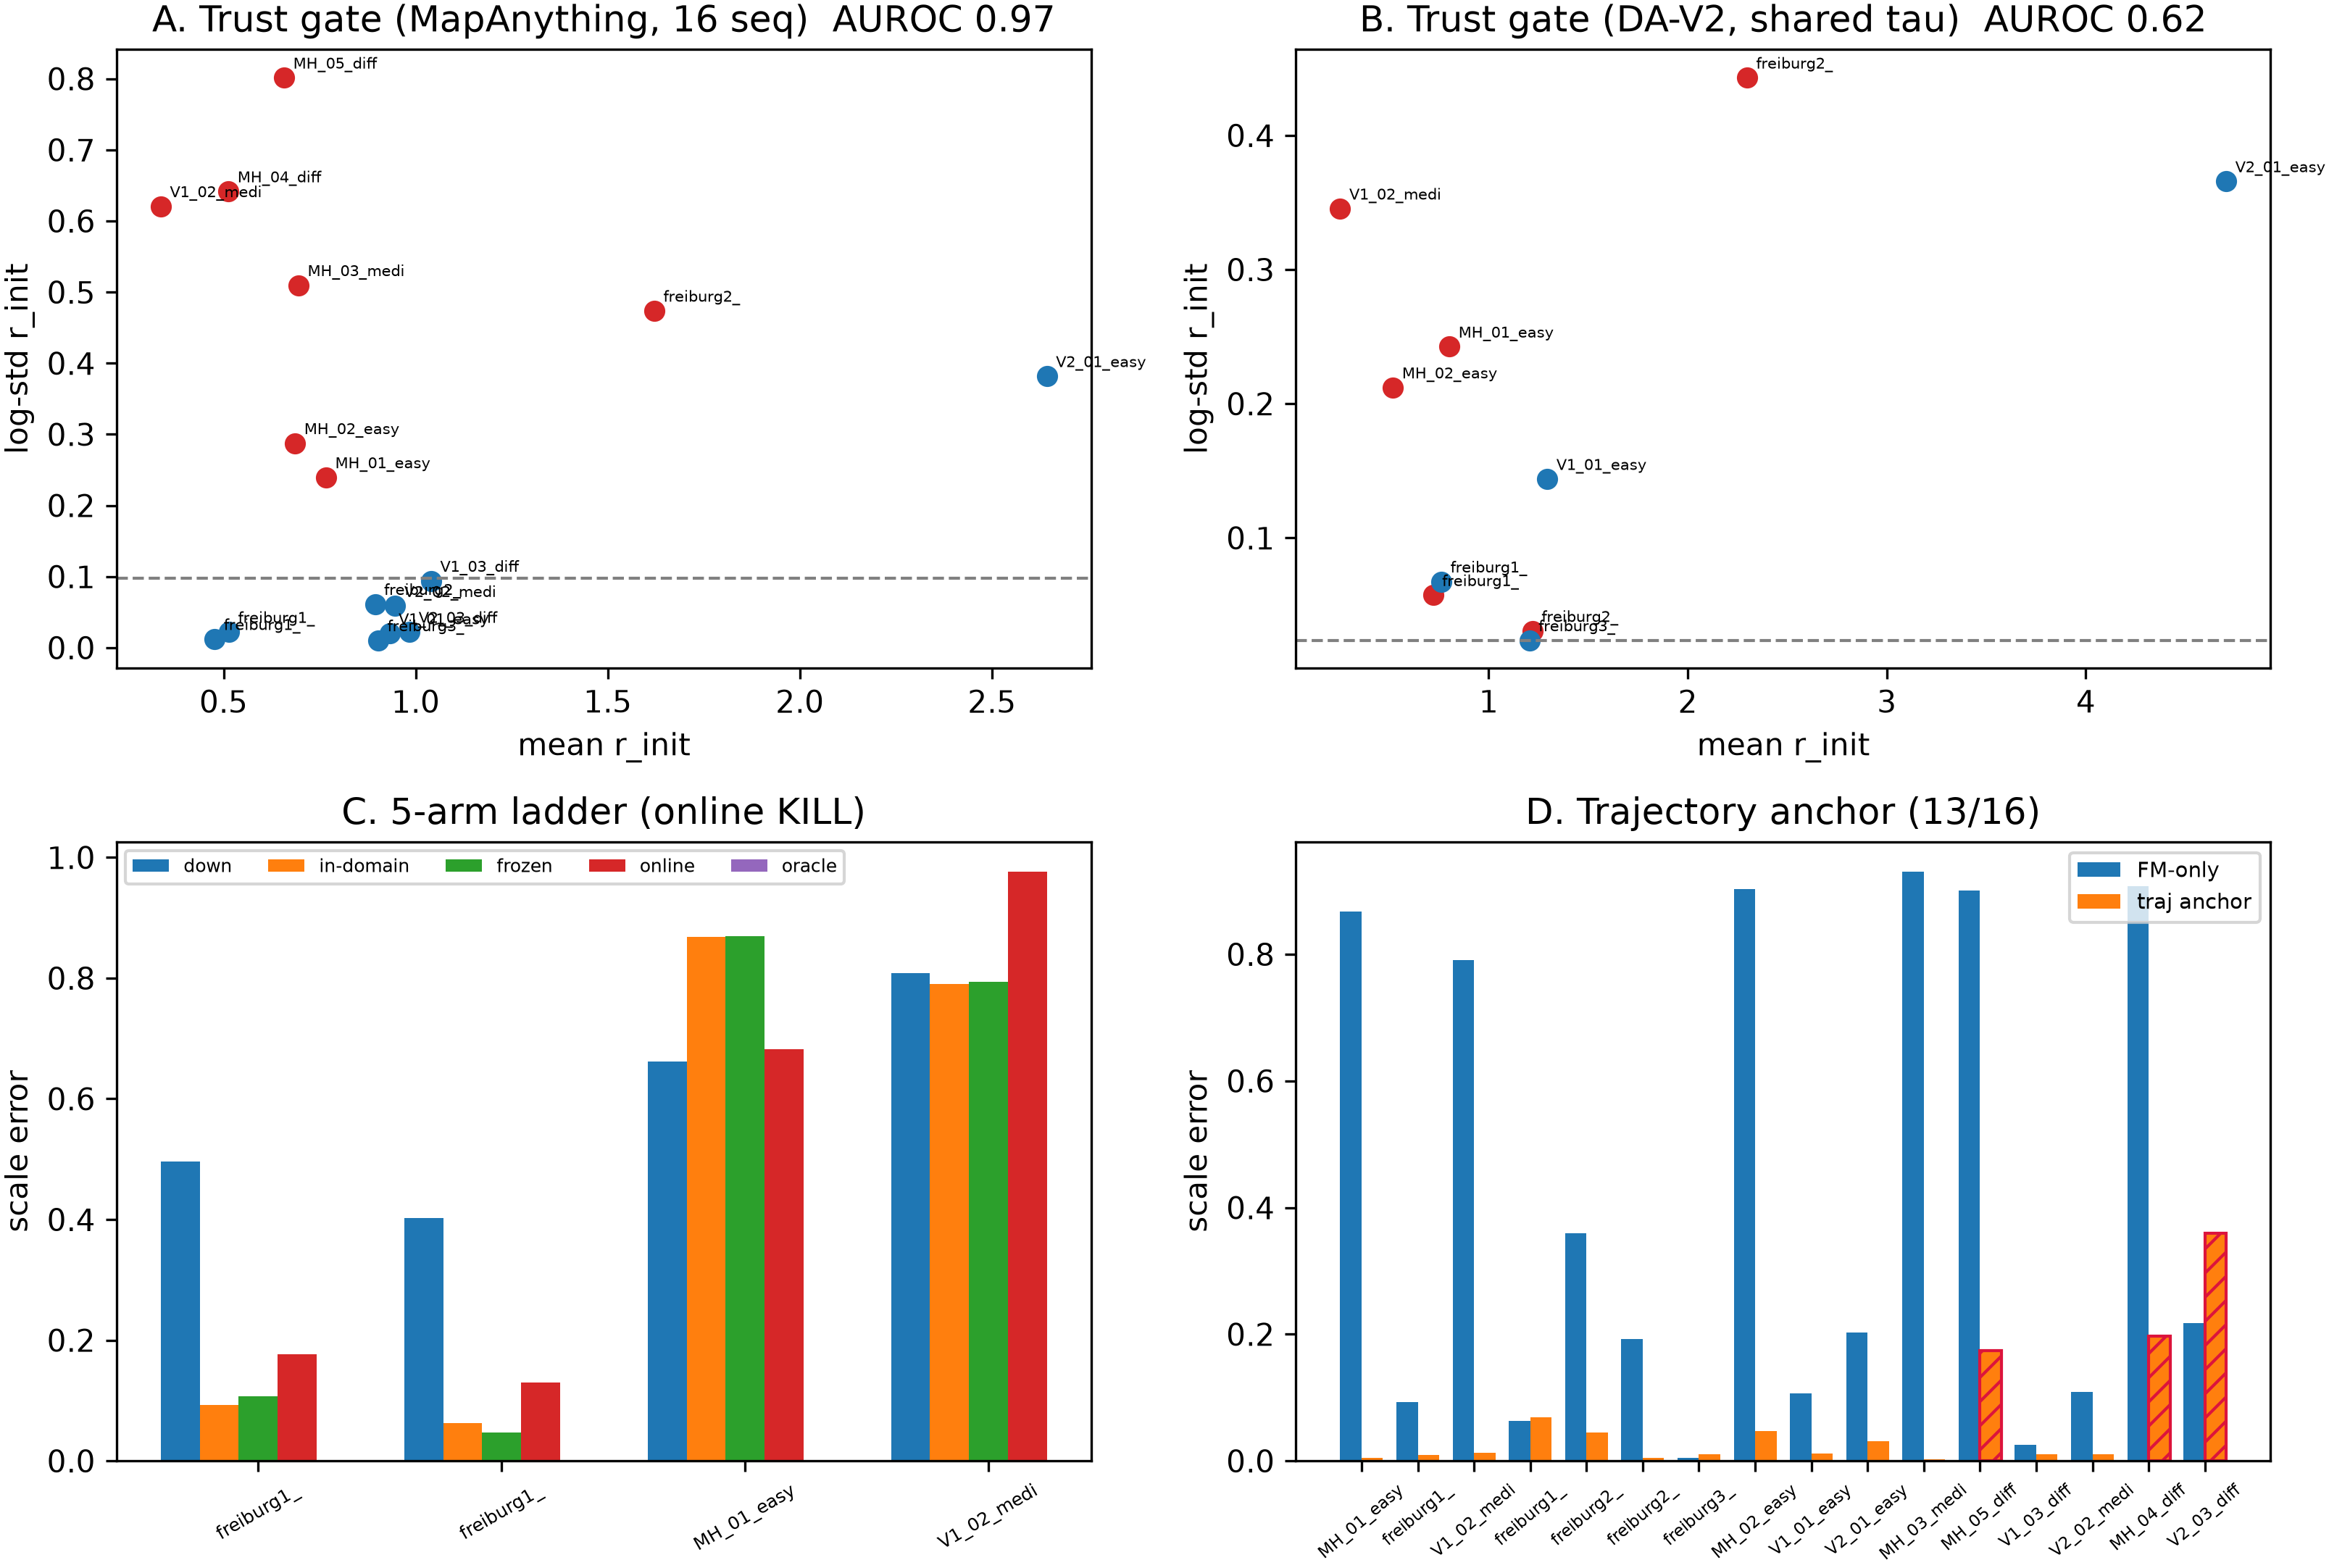
\includegraphics[width=0.76\linewidth]{caliprior_summary.png}
\caption{(A) trust gate, MapAnything, sixteen sequences (AUROC 0.97); (B) trust
gate, DA-V2 Metric at a shared threshold (AUROC 0.62; the gate is
model-specific); (C) the five-arm ladder (the online route we rejected); (D)
trajectory anchor versus teacher-only across sixteen sequences; the hatched bars
are the three sequences the anchor rejects.}
\label{fig:summary}
\end{figure}

\begin{figure}[t]
\centering
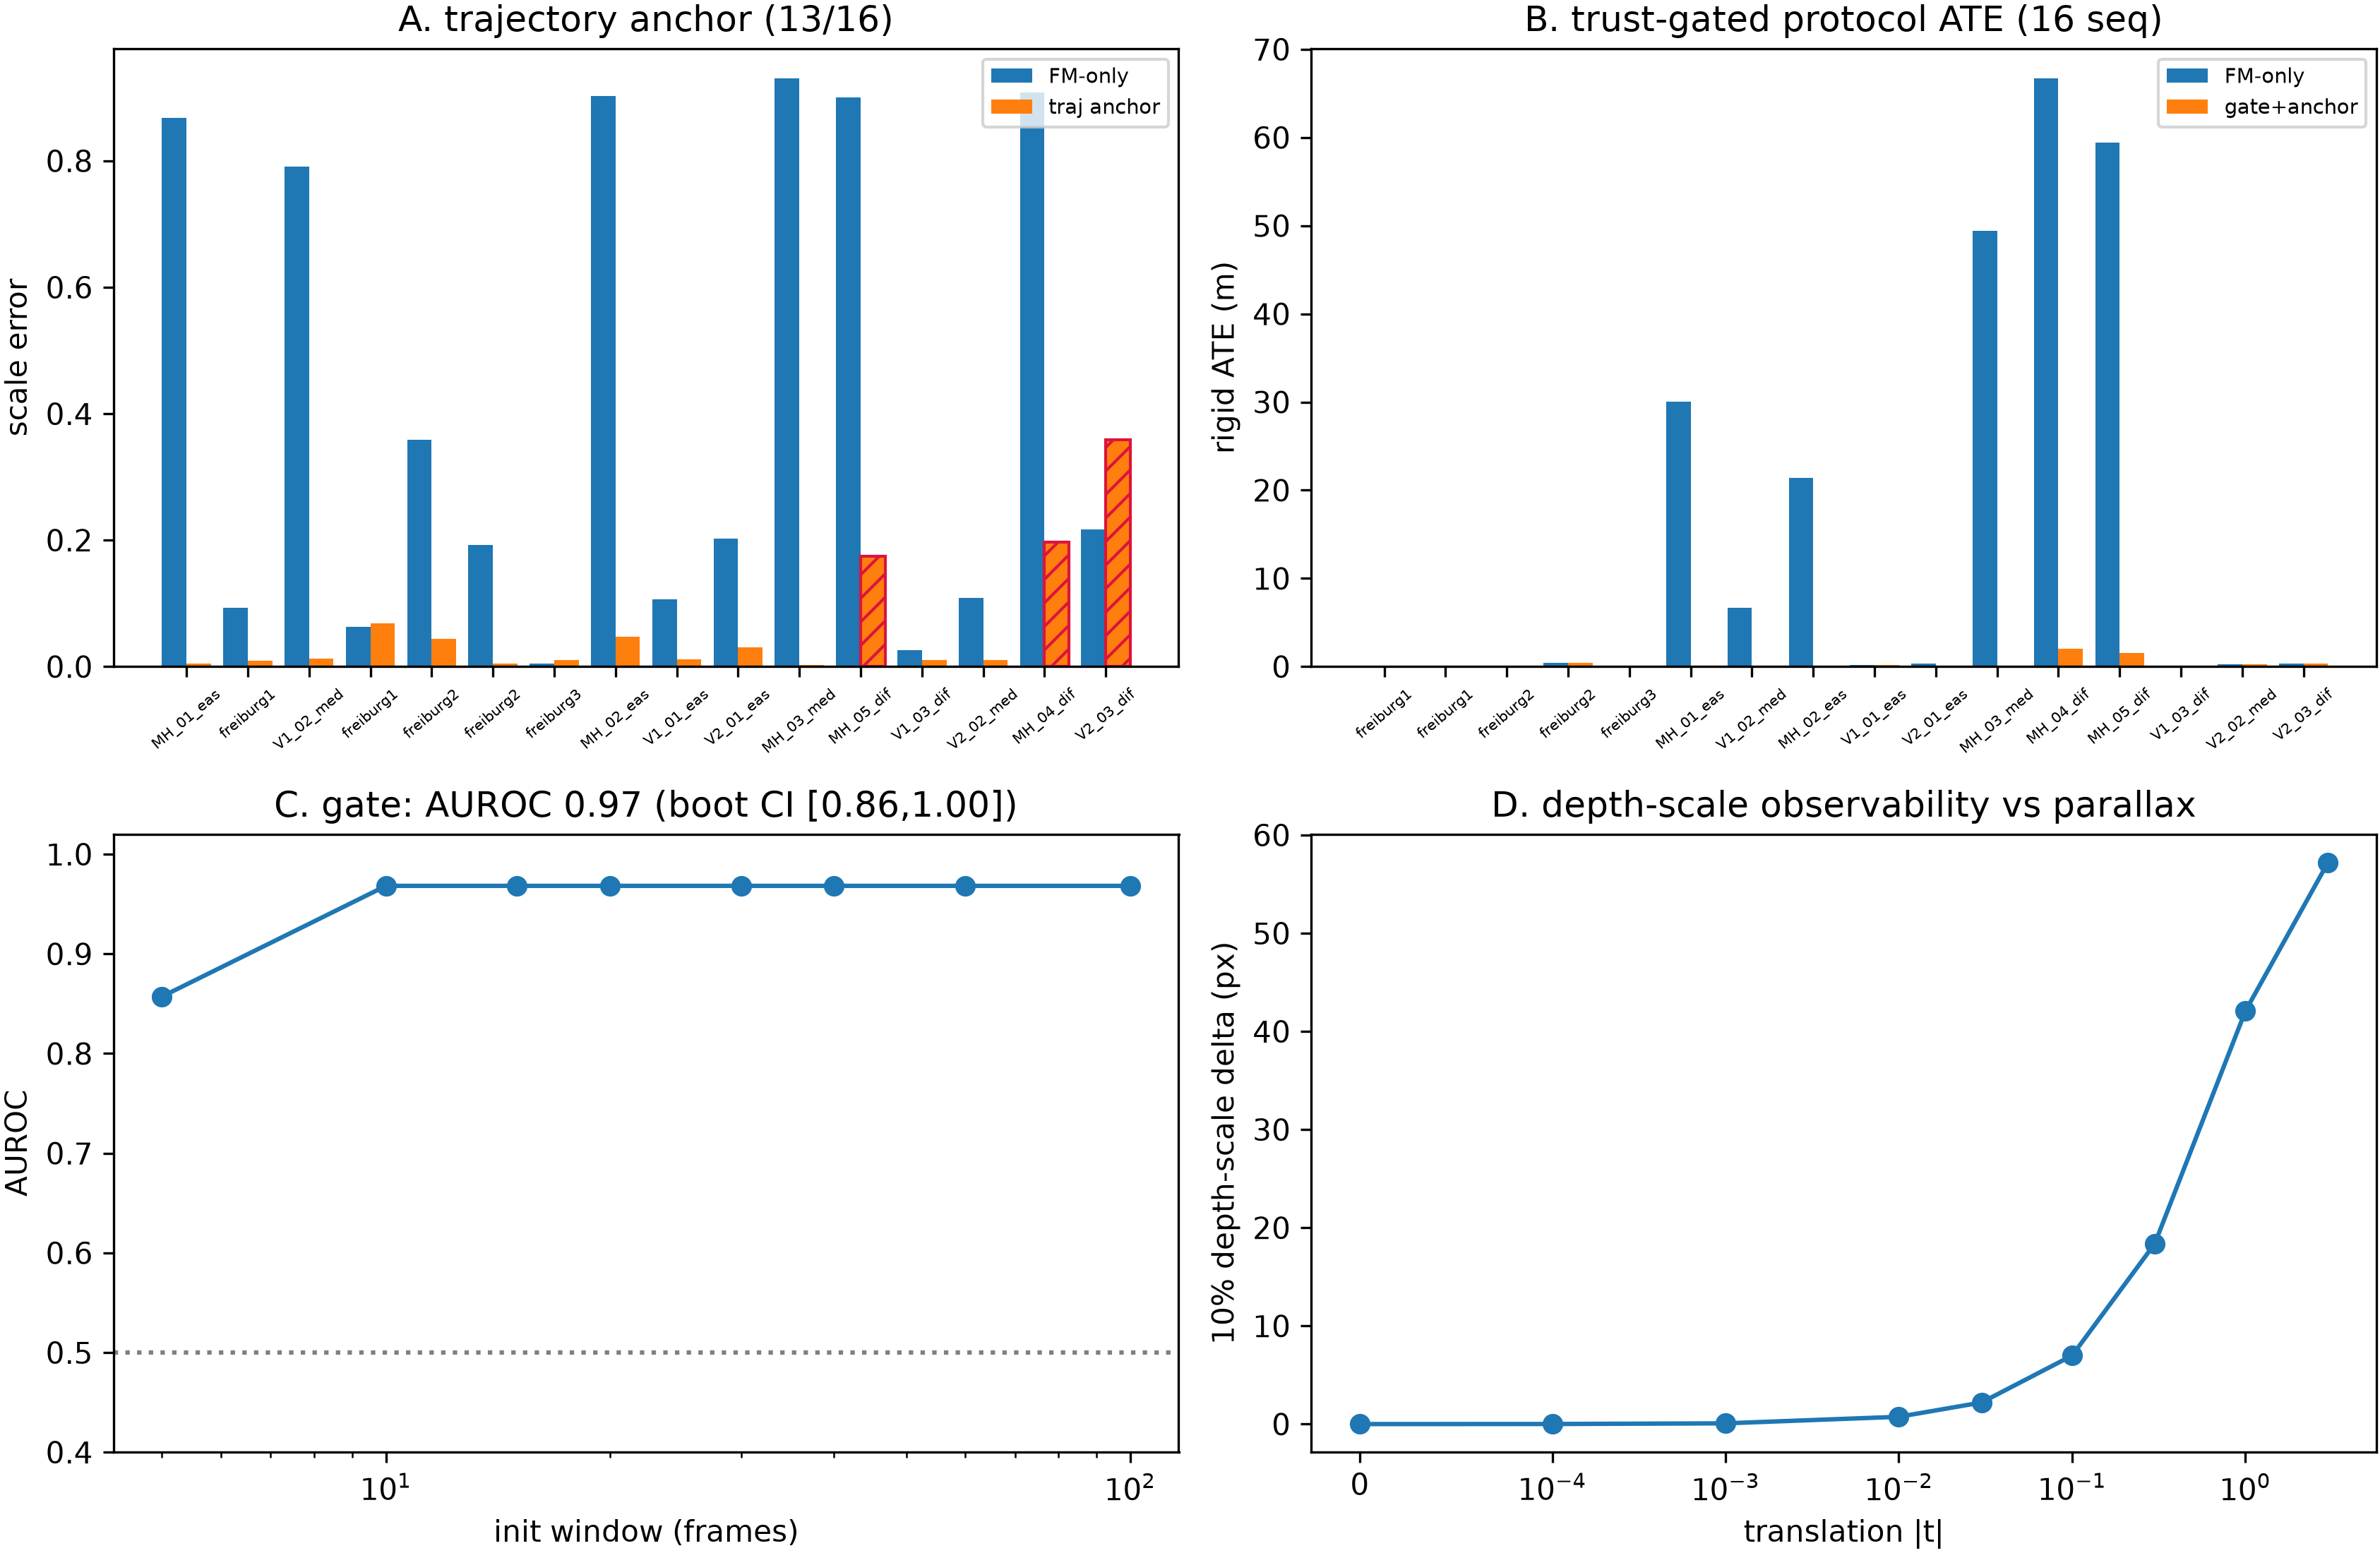
\includegraphics[width=0.76\linewidth]{caliprior_tier12.png}
\caption{(A) trajectory anchor versus teacher-only, sixteen sequences (13
accepted); (B) trust-gated protocol error across sixteen sequences, teacher-only
versus gate+anchor; (C) gate init-window sweep with bootstrap interval (sixteen
sequences); (D) depth-scale visibility versus parallax.}
\label{fig:tier12}
\end{figure}

\begin{figure}[t]
\centering
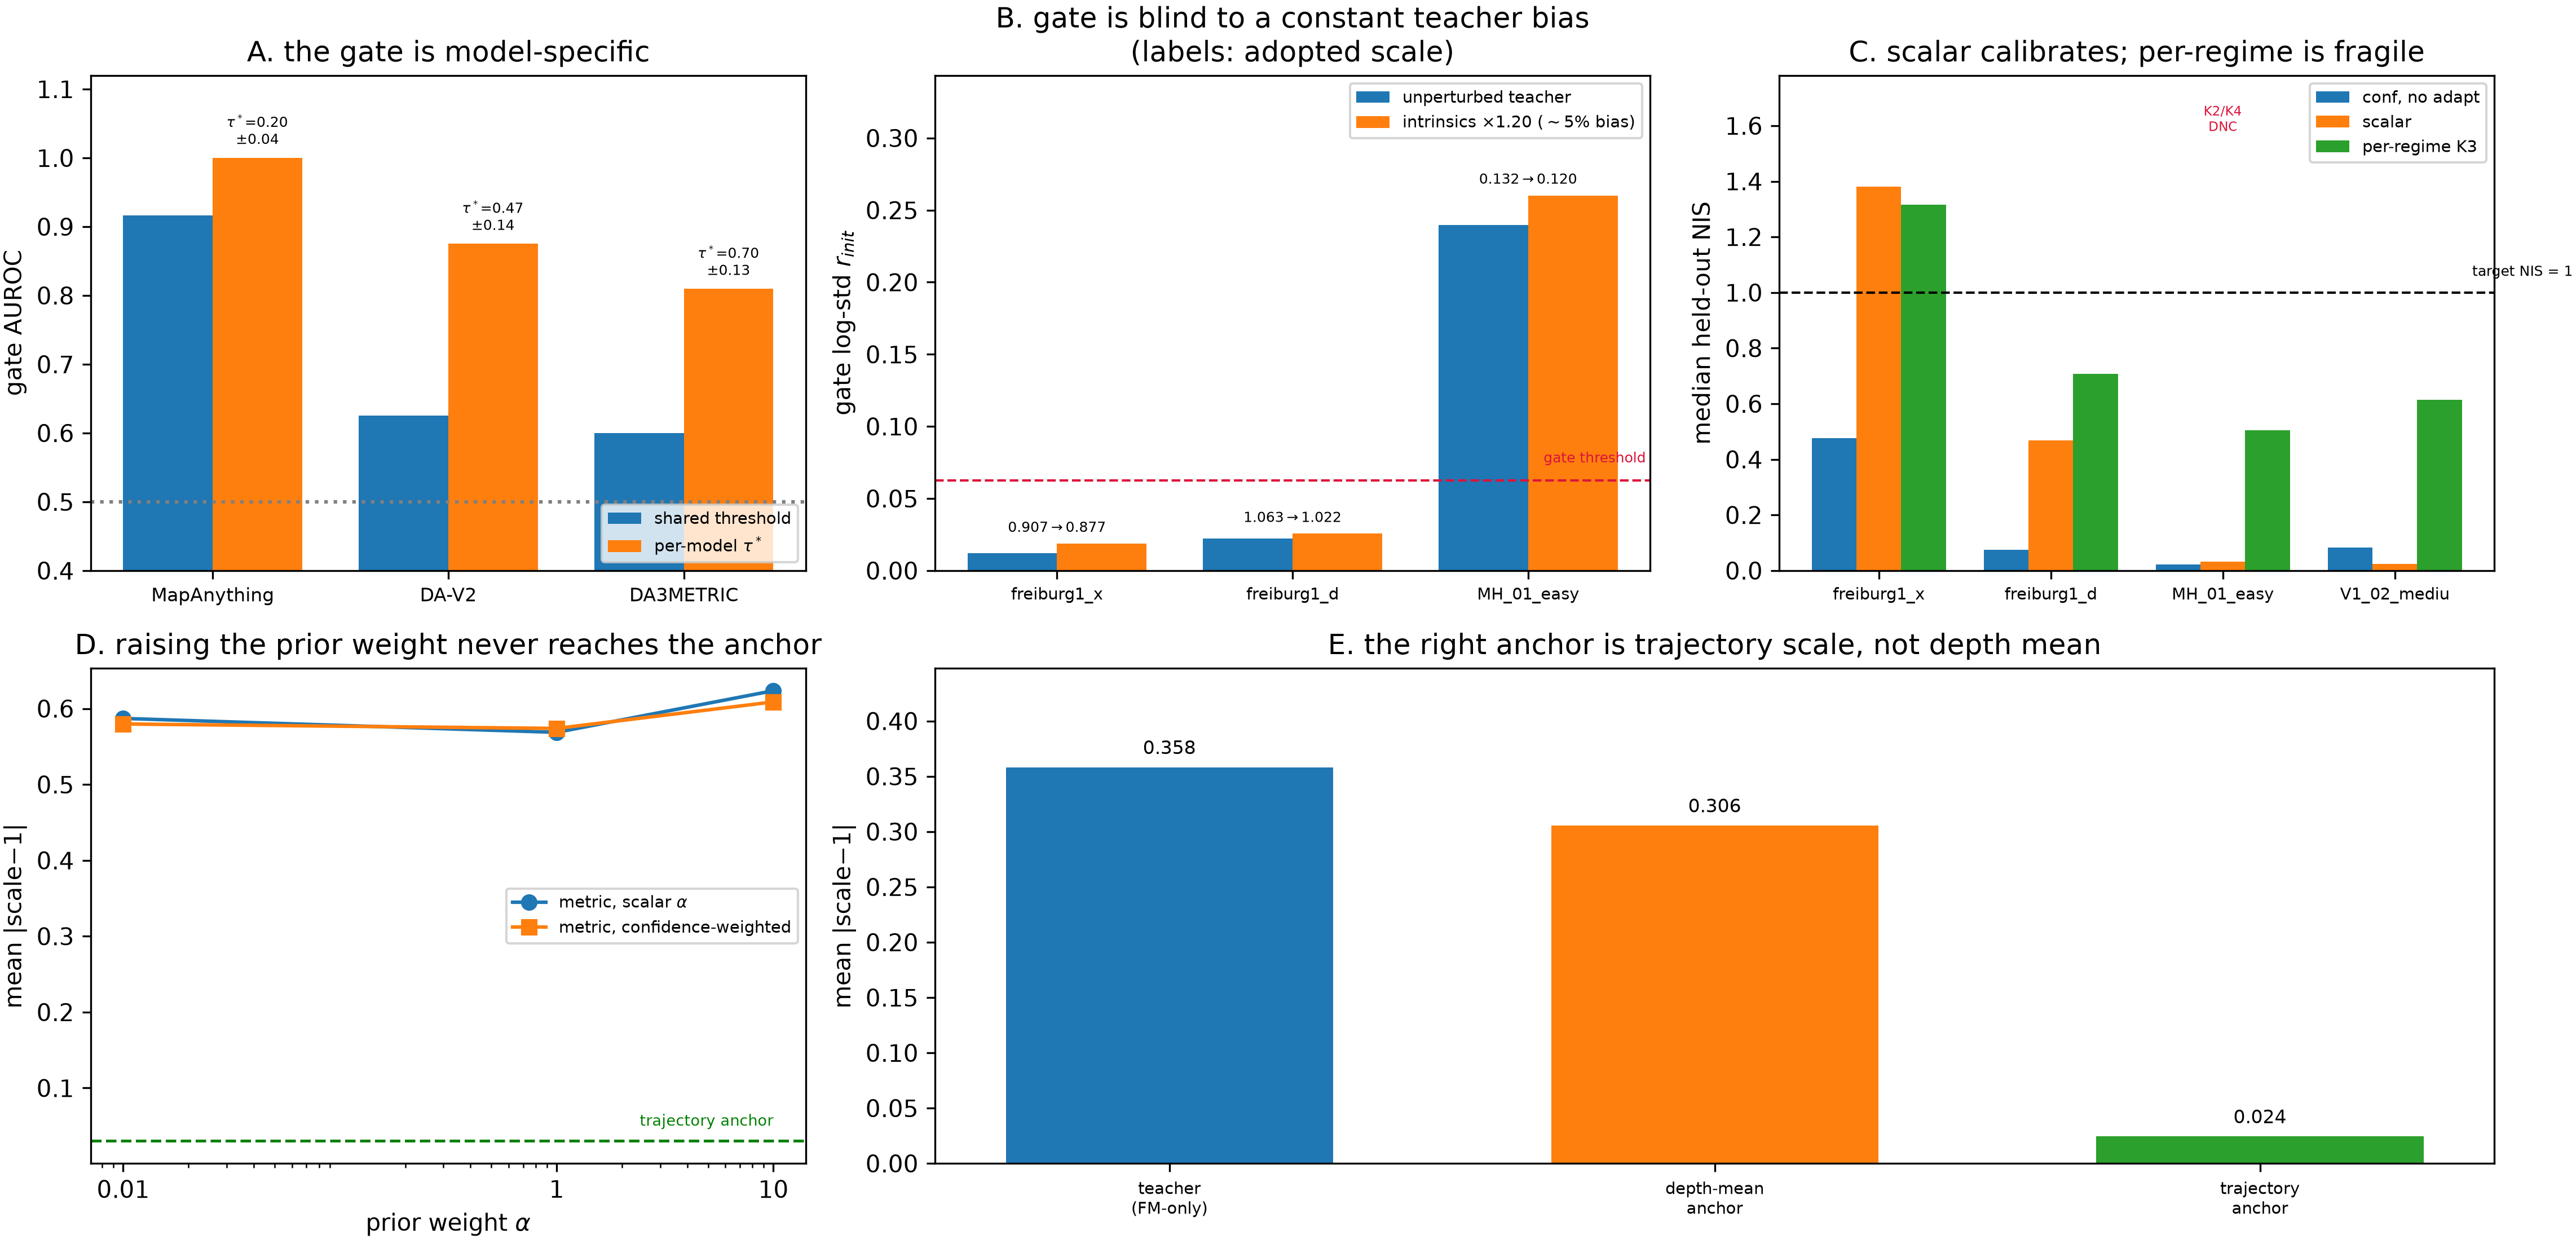
\includegraphics[width=\linewidth]{caliprior_mechanisms.png}
\caption{The five results stated above, shown together: (A) the gate is
model-specific: a per-model threshold lifts DA-V2/DA3METRIC to 0.88/0.81 but
at unstable $\tau^*$ (LOSO std 0.14/0.13), while MapAnything reaches 1.00 at a
stable $\tau^*=0.20$; (B) the gate is blind to a constant teacher bias; (C)
scalar adaptation reaches NIS $\approx 1$ while the per-regime extension is
fragile (K2/K4 did not converge unguarded); (D) raising the prior weight $\alpha$
through three orders of magnitude leaves the metric-factor arms near mean
$|\text{scale}-1|\approx0.6$, far from the trajectory anchor's 0.03; (E) of the
three anchors only the trajectory one works: teacher-only 0.358, depth-mean
0.306, trajectory 0.024 mean $|\text{scale}-1|$ over ten sequences.}
\label{fig:mechanisms}
\end{figure}
\section{Discussion and Limitations}
\label{sec:discussion}

\paragraph{Why the free-signal route fails.} The reference used by $r_{init}$ is
itself only up-to-scale, so the relation between $r$ and the needed correction
requires a domain-independent reference gauge that monocular geometry does not
provide. This is the observability statement, not a bug in our implementation.

\paragraph{Two halves of the error; scale is not adaptive.} Corollary~1 splits
the prior's error into a part the residuals can see (per-pixel $\sigma$, the
relative scale across keyframes, the shape) and a part they cannot: the single
global scale direction. A scalar part of the observable half is a legitimate
target for online estimation and consistency checking (Sec.~\ref{sec:observable}); the unobservable
half cannot be estimated at
all and must instead be \emph{gated} and \emph{anchored} by an external reference.
This is why the two constructive pieces do not overlap, and why the honest framing
for the global direction is one-shot identifiability plus an anchor, not
adaptive recovery of scale. Depth-channel consistency checks are \emph{circular}
for absolute scale (the prior defines the scale they would validate), and
image-channel residuals are blind to the joint rescale (Proposition~1): an
adaptive estimator can certify only what the gauge lets it see.

\paragraph{Practical protocol.} (1) Gate the model's metric scale on the
dispersion of the prior-free warm-up ratio. (2) If trusted, anchor the gauge to
the model. (3) Otherwise pin trajectory scale with a metric translation and use
the model for dense structure only; a depth-mean anchor is not sufficient.

\paragraph{What generalizes, and what does not.} The gauge diagnosis
(Corollary~1) and the trajectory anchor hold across the three depth models and
both in- and out-of-distribution domains; these are the transferable results. The
trust gate does not: the dispersion of the initial ratio separates scale errors
for MapAnything (AUROC 0.97) but not for DA-V2 (0.62) or DA3METRIC (0.60), and
model-internal confidence is useless everywhere we looked (0.44, or a constant
1.0). General GT-free detection of metric-scale uncertainty is therefore an open
problem, not a solved one.

\paragraph{What would falsify this.} The diagnosis fails if a purely monocular
residual changes under a joint $(t,z)$ rescale; none does, and the numeric
certificate checks the reprojection term. The anchor's universality fails if a
depth-mean or model-internal anchor matches its accuracy across domains; on our
ten sequences it does not (0.306 and 0.358 versus 0.024). The gate's
model-specificity fails if some model's dispersion ranks scale error well across
domains; for DA-V2 and DA3METRIC it does not (AUROC 0.62 and 0.60).

\paragraph{Limitations.} Sixteen sequences (five TUM, eleven EuRoC), three metric
models, one SLAM system. The six added EuRoC reference runs use a GS-free,
300-frame vehicle configuration (the Gaussian backend crashes on some of those
visuals), so that part of the gate comparison is across a slightly different
backend setup. The gate is model-specific and must be validated per model; it
detects teacher inconsistency, not a constant bias, which by construction leaves
the gate statistic unchanged (Sec.~\ref{sec:observable}), so a globally biased teacher must be
caught by the anchor. Local-drift testing is on TUM only (EuRoC has no dense
ground-truth depth); the trajectory anchor still needs an external metric sensor,
and it recovers 13 of the 16 sequences, refusing the three difficult EuRoC
sequences where matched translation is too poor to certify a scale; the
sixteen-sequence gate and protocol figures include those failures rather than
excluding them. KITTI is reported as a limit of the SLAM system, not a result
about depth models.
The per-regime $\sigma$ of Sec.~\ref{sec:observable} passes the pre-registered test in one
configuration but is \textbf{not robust}: K2/K4 hung unguarded and a stability
guard erased the calibration gain, so only the scalar adaptation is reported as a
mechanism. A deliberate local FM step is likewise absorbed by the metric-factor
vehicle (Sec.~\ref{sec:nolocal}), so we report no live local lever.

\section{Conclusion}

A frozen FM metric-depth prior does not transfer metric scale to monocular SLAM
on its own. The monocular gauge makes the \emph{global} scale direction
unobservable (Corollary~1), and the system as shipped normalizes away even local
model scale per keyframe. The diagnosis is implementation-independent: it is
confirmed after those normalizations are removed (Sec.~\ref{sec:nolocal}), so it is a property of
the monocular factor graph, not of one codebase. For the global direction the fix
is one external metric
anchor plus a GT-free trust gate, and no cleverer bias or covariance estimator can
substitute. This is a statement about scale, not about adaptation in general: a
scalar variance scale on the observable half can be calibrated online, though a
per-regime refinement was not robust, provided neither is mistaken for scale
recovery. We give the measured chain and a minimal protocol.

